\documentclass[tikz]{standalone}
\usepackage{tikz}
\usepackage{tikz-qtree}
\usetikzlibrary{shapes, trees,calc,positioning, arrows.meta}
\definecolor{Red}{HTML}{e32b2d}
\definecolor{Green}{HTML}{15821b}
\definecolor{Blue}{HTML}{0984e3}
\def\deft#1{\texttt{\textcolor{Blue}{#1}}}


\begin{document}
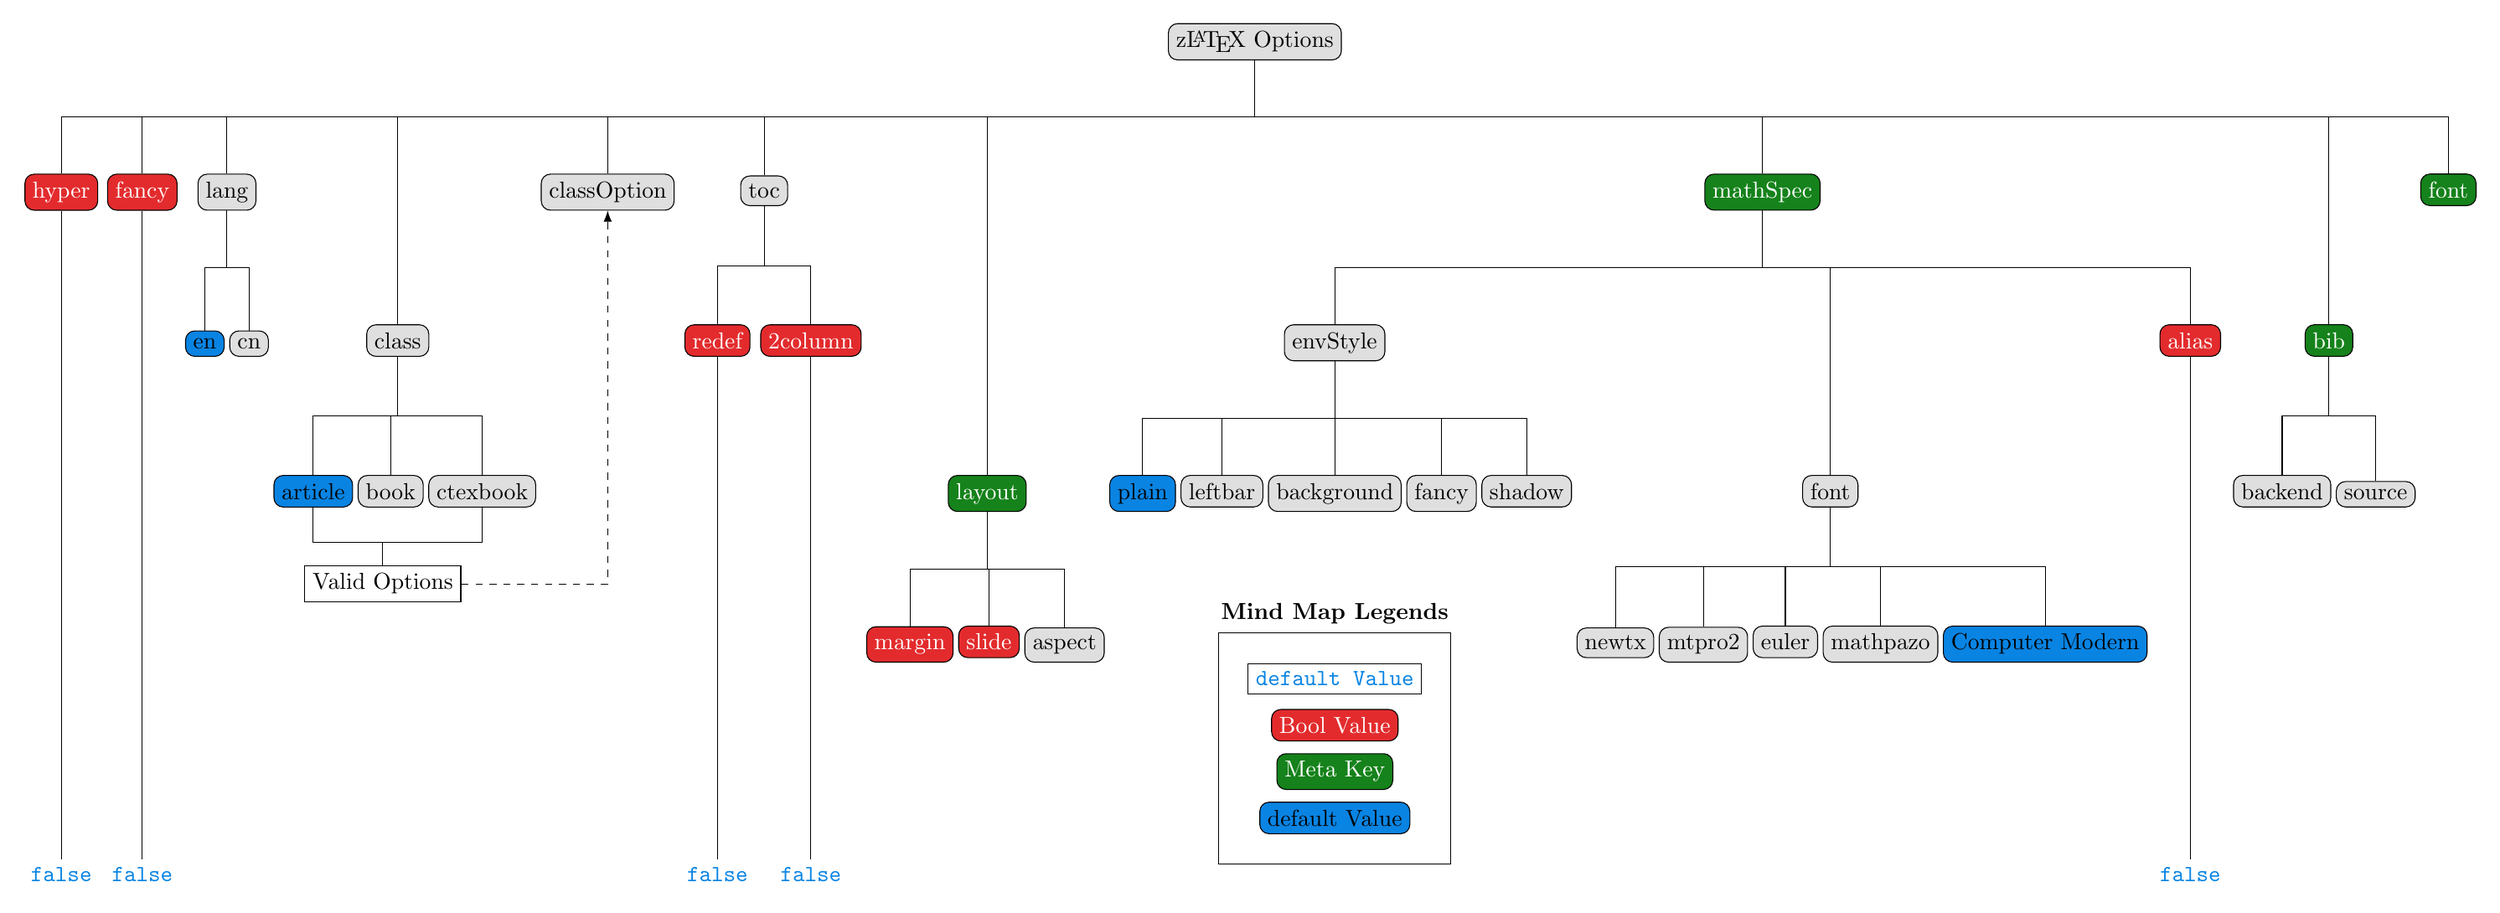
\begin{tikzpicture}[
    >=Latex,
    level distance=65,
    edge from parent/.style={draw, edge from parent fork down},
    frontier/.style={distance from root=360},
    normalKey/.style={draw, rectangle, rounded corners, fill=gray!25},
    boolKey/.style={draw, rectangle, rounded corners, fill=Red, text=white},
    metaKey/.style={draw, rectangle, rounded corners, fill=Green, text=white},
  ]
  \Tree
    [.\node[normalKey] {z\LaTeX{} Options};
      [.\node[boolKey] {hyper}; \deft{false} ]
      [.\node[boolKey] {fancy}; \deft{false} ]
      [.\node[normalKey] {lang}; 
        [.\node[normalKey, fill=Blue] {en}; ]
        [.\node[normalKey] {cn}; ]
      ]
      [[.\node[normalKey] {class}; 
        [.\node[normalKey, fill=Blue] (articleL) {article};  ]
        [.\node[normalKey] {book};     ]
        [.\node[normalKey] (ctexbookR) {ctexbook}; ]
      ]]
      [.\node[normalKey] (classOptionC) {classOption};]
      [.\node[normalKey] {toc};
        [.\node[boolKey] {redef};   \deft{false} ]
        [.\node[boolKey] {2column}; \deft{false} ]
      ]
      [[[.\node[metaKey] {layout}; 
        [.\node[boolKey]   {margin}; ]
        [.\node[boolKey]   {slide};  ]
        [.\node[normalKey] {aspect}; ]
      ]]]
      [.\node[metaKey] {mathSpec};
        [.\node[normalKey] {envStyle}; 
            [.\node[normalKey, fill=Blue] {plain}; ]
            [.\node[normalKey] {leftbar};    ]
            [.\node[normalKey] (annotateC) {background}; ]
            [.\node[normalKey] {fancy};      ]
            [.\node[normalKey] {shadow};     ]
        ]
        [[.\node[normalKey] {font}; 
          [.\node[normalKey] {newtx}; ]
          [.\node[normalKey] {mtpro2}; ]
          [.\node[normalKey] {euler}; ]
          [.\node[normalKey] {mathpazo}; ]
          [.\node[normalKey, fill=Blue] {Computer Modern}; ]
        ]]
        [.\node[boolKey] {alias}; \deft{false} ]
      ]
      [[.\node[metaKey] {bib}; 
        [.\node[normalKey] {backend}; ]
        [.\node[normalKey] {source}; ]
      ]]
      [.\node[metaKey] {font}; ]
    ]
  % lines
  \draw (articleL.south) |- ++(0, -1.5em) -| (ctexbookR.south);
  \draw ($(articleL.south)+(3em, -2.5em)$)node[draw, rectangle, below] {Valid Options} -- ++(0, 1em);
  \draw[->, dashed] ($(articleL.south)+(6.4em, -3.3em)$) -| (classOptionC);
  % annotatations
  \node[text=Blue, rectangle, draw] at ($(annotateC)+(0, -8em)$)  {\texttt{default Value}};
  \node[boolKey] at ($(annotateC)+(0, -10em)$)  {Bool Value};
  \node[metaKey] at ($(annotateC)+(0, -12em)$)  {Meta Key};
  \node[metaKey, fill=Blue, text=black] at ($(annotateC)+(0, -14em)$)  {default Value};
  \draw ($(annotateC)+(-5em, -16em)$) rectangle ++(10em, 10em)node[right=-5em, above] {\textbf{Mind Map Legends}};
\end{tikzpicture}
\end{document}